\subsection{SP1: reclutamiento homogéneo mediante juegos poblacionales}
\label{sec:resultados-sp1-homogeneous}

\subsubsection{Unificación de SP0 y SP1}

El antiguo SP0 (asignación homogénea uno a uno) y el antiguo SP1
(reclutamiento por cuórum) son instancias del mismo problema. Se consideran $N$
robots homogéneos, $K$ cargas homogéneas y un cuórum común $q\geq1$, en el régimen
balanceado $N=Kq$. Cada robot elige una sola carga y cada carga debe recibir
exactamente $q$ robots. El caso $q=1$ recupera el emparejamiento uno a uno; $q>1$
representa reclutamiento cooperativo. Desde este capítulo, ambos casos constituyen
un único SP1. Los directorios históricos se conservan únicamente por trazabilidad.

Sea $x_{ik}\in[0,1]$ la preferencia del robot $i$ por la carga $k$, con
$\sum_k x_{ik}=1$, y sea $n_k(x)=\sum_i x_{ik}$ la ocupación. Para el coste
normalizado $c_{ik}$ se propone el potencial
\begin{equation}
 \Phi(x)=-\frac{\alpha}{2}\sum_{k=1}^{K}\bigl(n_k(x)-q\bigr)^2
         -\beta\sum_{i=1}^{N}\sum_{k=1}^{K}c_{ik}x_{ik},
 \label{eq:sp1-potential}
\end{equation}
con $\alpha,\beta>0$. Su gradiente define el fitness individual
\begin{equation}
 f_{ik}(x)=\frac{\partial\Phi}{\partial x_{ik}}
          =-\alpha\bigl(n_k(x)-q\bigr)-\beta c_{ik}.
 \label{eq:sp1-fitness}
\end{equation}
El primer término penaliza coaliciones incompletas o sobreocupadas y el segundo
prefiere asignaciones cercanas. Esta construcción traslada a robótica móvil la
lectura de juegos poblacionales y control distribuido de
\citet{quijano2017population,martinez2020formation,martinezpiazuelo2022tcss}.

\subsubsection{Protocolos y resultados teóricos}

Se implementan tres protocolos continuos. Para cada robot, Smith mueve masa desde
$\ell$ hacia $k$ cuando $f_{ik}>f_{i\ell}$:
\begin{equation}
 \dot x_{ik}=\sum_{\ell}x_{i\ell}[f_{ik}-f_{i\ell}]_+
 -x_{ik}\sum_{\ell}[f_{i\ell}-f_{ik}]_+ .
 \label{eq:sp1-smith}
\end{equation}
El replicador usa $\dot x_{ik}=x_{ik}(f_{ik}-\bar f_i)$ y BNN usa
$\dot x_{ik}=[f_{ik}-\bar f_i]_+-x_{ik}\sum_\ell[f_{i\ell}-\bar f_i]_+$,
donde $\bar f_i=\sum_kx_{ik}f_{ik}$. Estos protocolos comparten el mismo juego;
la comparación evalúa la ley de revisión, no payoffs distintos.

\begin{proposicion}[Invariancia del símplex]
Para Smith, replicador y BNN, $\sum_k\dot x_{ik}=0$ para todo robot $i$; además,
el campo no dirige una componente nula hacia valores negativos. Por tanto,
$x_i(0)\in\Delta^K$ implica $x_i(t)\in\Delta^K$.
\end{proposicion}
\begin{proof}
En los tres campos los términos de entrada y salida se cancelan al sumar sobre
estrategias. En la frontera, Smith y BNN conservan términos de entrada no negativos
y el replicador anula la componente mediante el factor $x_{ik}$.
\end{proof}

\begin{proposicion}[Ascenso de potencial para Smith]
Bajo ocupación exacta, el campo de Smith satisface
\begin{equation}
 \dot\Phi=\sum_i\sum_{k,\ell}x_{i\ell}
 [f_{ik}-f_{i\ell}]_+^2\geq0.
 \label{eq:sp1-potential-ascent}
\end{equation}
Todo punto estacionario satisface la condición de soporte de Nash:
$x_{ik}>0\Rightarrow f_{ik}\geq f_{i\ell}$ para toda $\ell$.
\end{proposicion}
\begin{proof}
Por la regla de la cadena, $\dot\Phi=\sum_{i,k}f_{ik}\dot x_{ik}$.
Al sustituir~\eqref{eq:sp1-smith}, intercambiar $k$ y $\ell$ en el término de
salida y agrupar, se obtiene~\eqref{eq:sp1-potential-ascent}. La igualdad exige
que no exista una migración rentable desde una estrategia con masa positiva.
\end{proof}

Para información exacta, los otros campos también son compatibles con el potencial:
el replicador satisface $\dot\Phi=\sum_{i,k}x_{ik}(f_{ik}-\bar f_i)^2\geq0$
y BNN satisface $\dot\Phi=\sum_{i,k}[f_{ik}-\bar f_i]_+^2\geq0$.
La diferencia está en los conjuntos estacionarios: el replicador puede quedar inmóvil
en una cara que excluya una estrategia mejor, mientras Smith y BNN permiten entrada
desde componentes nulas.

\begin{proposicion}[Equilibrio y óptimo continuo]
La función $\Phi$ es cóncava sobre $\prod_i\Delta^K$. En consecuencia, todo
perfil que cumple la condición completa de soporte de Nash es un máximo global de
la relajación continua de~\eqref{eq:sp1-potential}. El recíproco también se cumple
por las condiciones KKT. Este óptimo continuo no implica optimalidad entera.
\end{proposicion}
\begin{proof}
El término cuadrático es el negativo de una suma de cuadrados de funciones afines
y el término espacial es lineal; por tanto, $\Phi$ es cóncava. La condición de
soporte de Nash coincide con las condiciones KKT en el producto de símplex. Para
una función cóncava diferenciable, dichas condiciones son suficientes y necesarias
para optimalidad global continua.
\end{proof}

Hay, por tanto, tres niveles que no deben confundirse: el equilibrio Nash del juego
continuo; el máximo global de su potencial cóncavo; y el óptimo entero con exactamente
$q$ robots por carga. Los dos primeros coinciden bajo la condición completa de soporte,
pero el tercero exige cierre discreto. Entre asignaciones enteras ya balanceadas, el
húngaro expandido minimiza la distancia bajo los supuestos balanceados declarados; QR produce una asignación cardinal válida, sin aportar optimalidad.

Estas garantías son continuas y requieren ocupación exacta. La implementación de
Euler usa un reescalado temporal positivo por robot para acotar la tasa de revisión;
no altera puntos estacionarios ni el signo continuo. La auditoría confirmó cero
violaciones discretas del potencial en las 450 ejecuciones Smith con grafo completo.
Con un anillo y cuatro rondas de consenso, la ocupación es aproximada: se mide la
sensibilidad, pero no se reclama monotonía ni convergencia teórica.

La preferencia continua no es todavía una coalición ejecutable. Se conserva un
registro RAW mediante $\arg\max_kx_{ik}$ y, como etapa separada, un cierre entero
QR que procesa preferencias y llena $q$ plazas por carga. En $N=Kq$ y con todos
los pares admisibles, el cierre termina con una asignación válida porque cada
aceptación reduce en una unidad el número finito de plazas libres. Esta propiedad
solo asegura factibilidad cardinal bajo los supuestos; no prueba que QR sea distribuido u óptimo.
La cota exacta centralizada expande cada carga en $q$ plazas y aplica el algoritmo
húngaro \citep{kuhn1955hungarian}.

\subsubsection{Diseño experimental reproducible}

La campaña confirmatoria \texttt{SP1\_HOMOGENEOUS\_v1\_1} cruza
$N\in\{8,16,24\}$, $q\in\{1,2\}$, tres geometrías (uniforme, agrupada y
cruzada), dos grafos fijos (completo y anillo) y 25 réplicas: 900 mundos y
7200 ejecuciones. Las semillas 330000--330899 se abrieron después de congelar
factores, payoffs, métodos e hipótesis. Cada mundo es compartido por los ocho
tratamientos. El piloto v1 queda excluido porque su paso de Euler violó la
auditoría predeclarada; la repetición usa semillas nuevas y no cambia el payoff.

Los tratamientos son Smith, replicador y BNN seguidos del mismo cierre QR;
preferencia uniforme+QR y aleatoria+QR como controles del cierre; greedy;
una subasta proxy; y el húngaro expandido como óptimo centralizado. Se reportan
RAW y CLOSED por separado, regret normalizado respecto al óptimo, distancia,
residuo, convergencia al umbral, ganancia de potencial, mensajes y tiempo.
Los cinco contrastes Smith--referencia son pareados por mundo, con bootstrap del
95\% y corrección de Holm.

\begin{figure}[H]
\centering
\begin{minipage}[t]{0.49\textwidth}
\centering
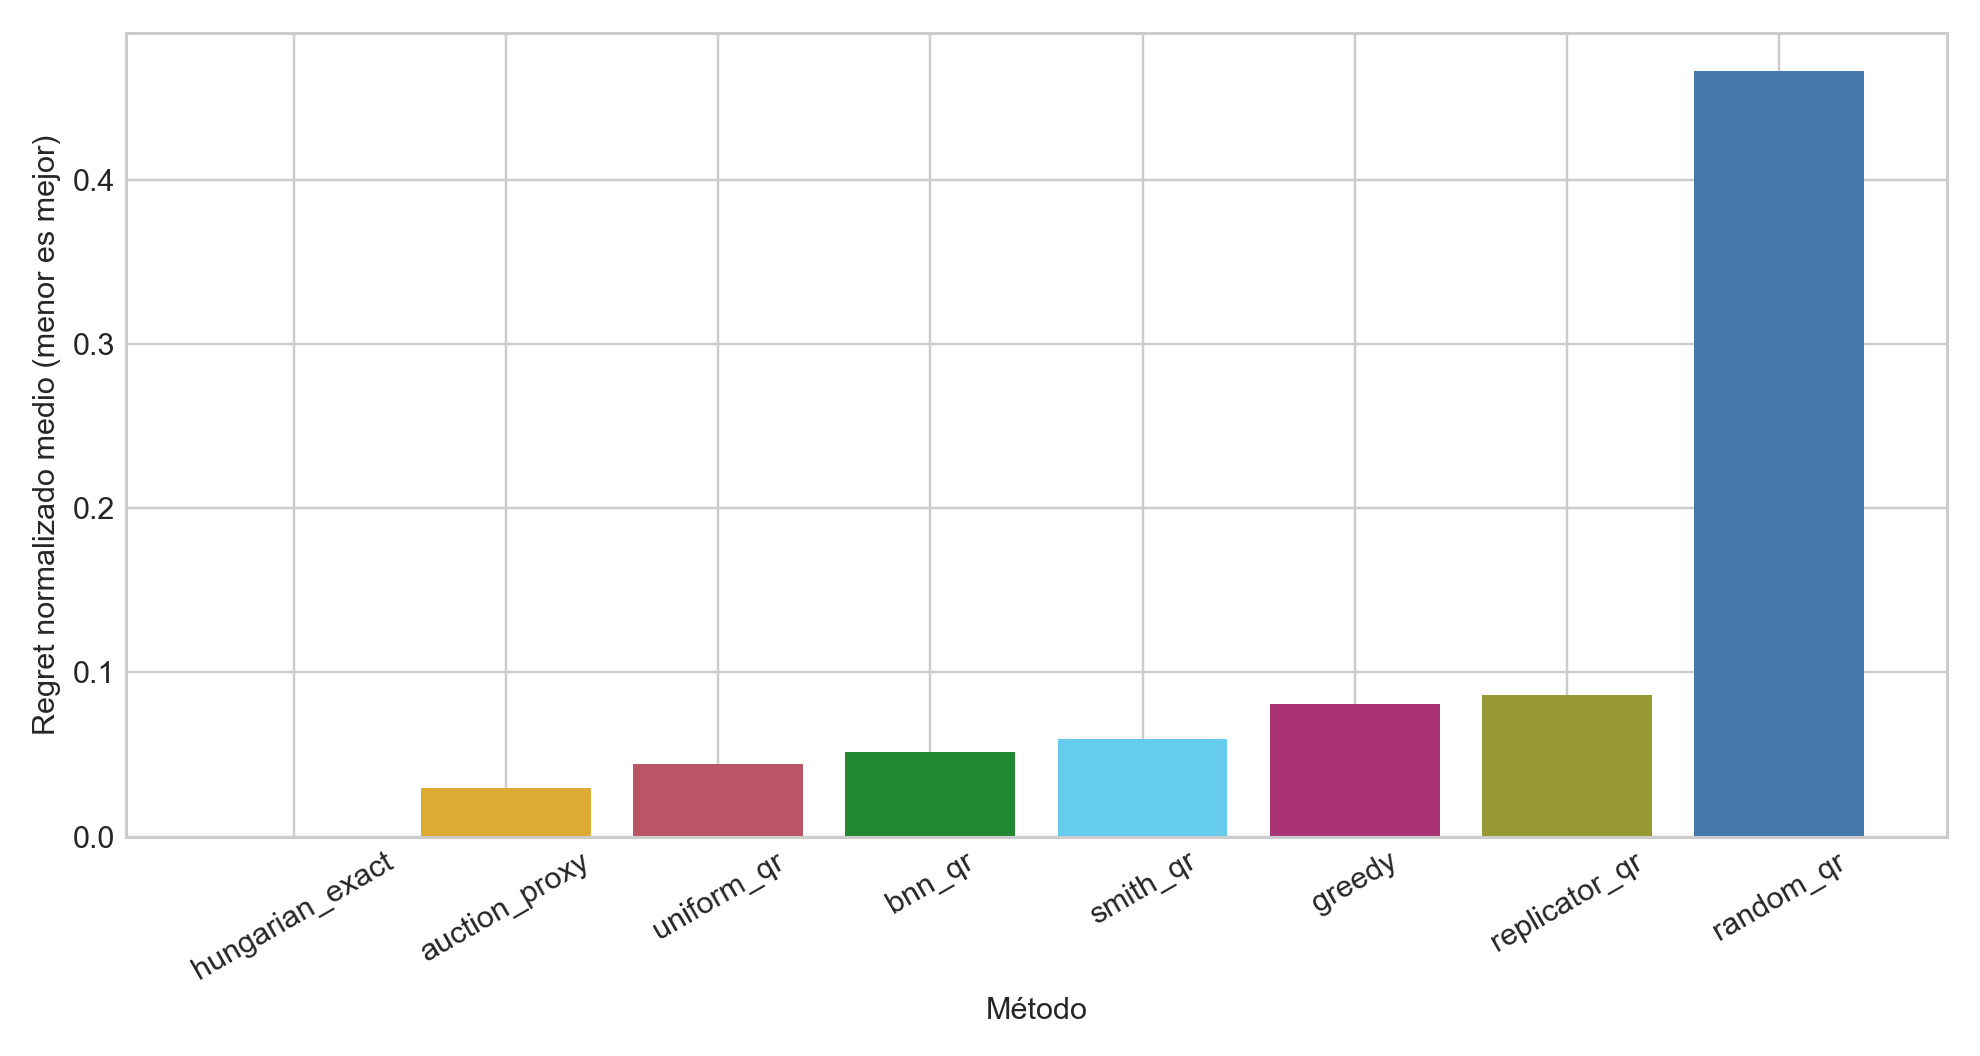
\includegraphics[width=\linewidth]{figures/fig-sp1-homogeneous-regret.png}
\end{minipage}\hfill
\begin{minipage}[t]{0.49\textwidth}
\centering
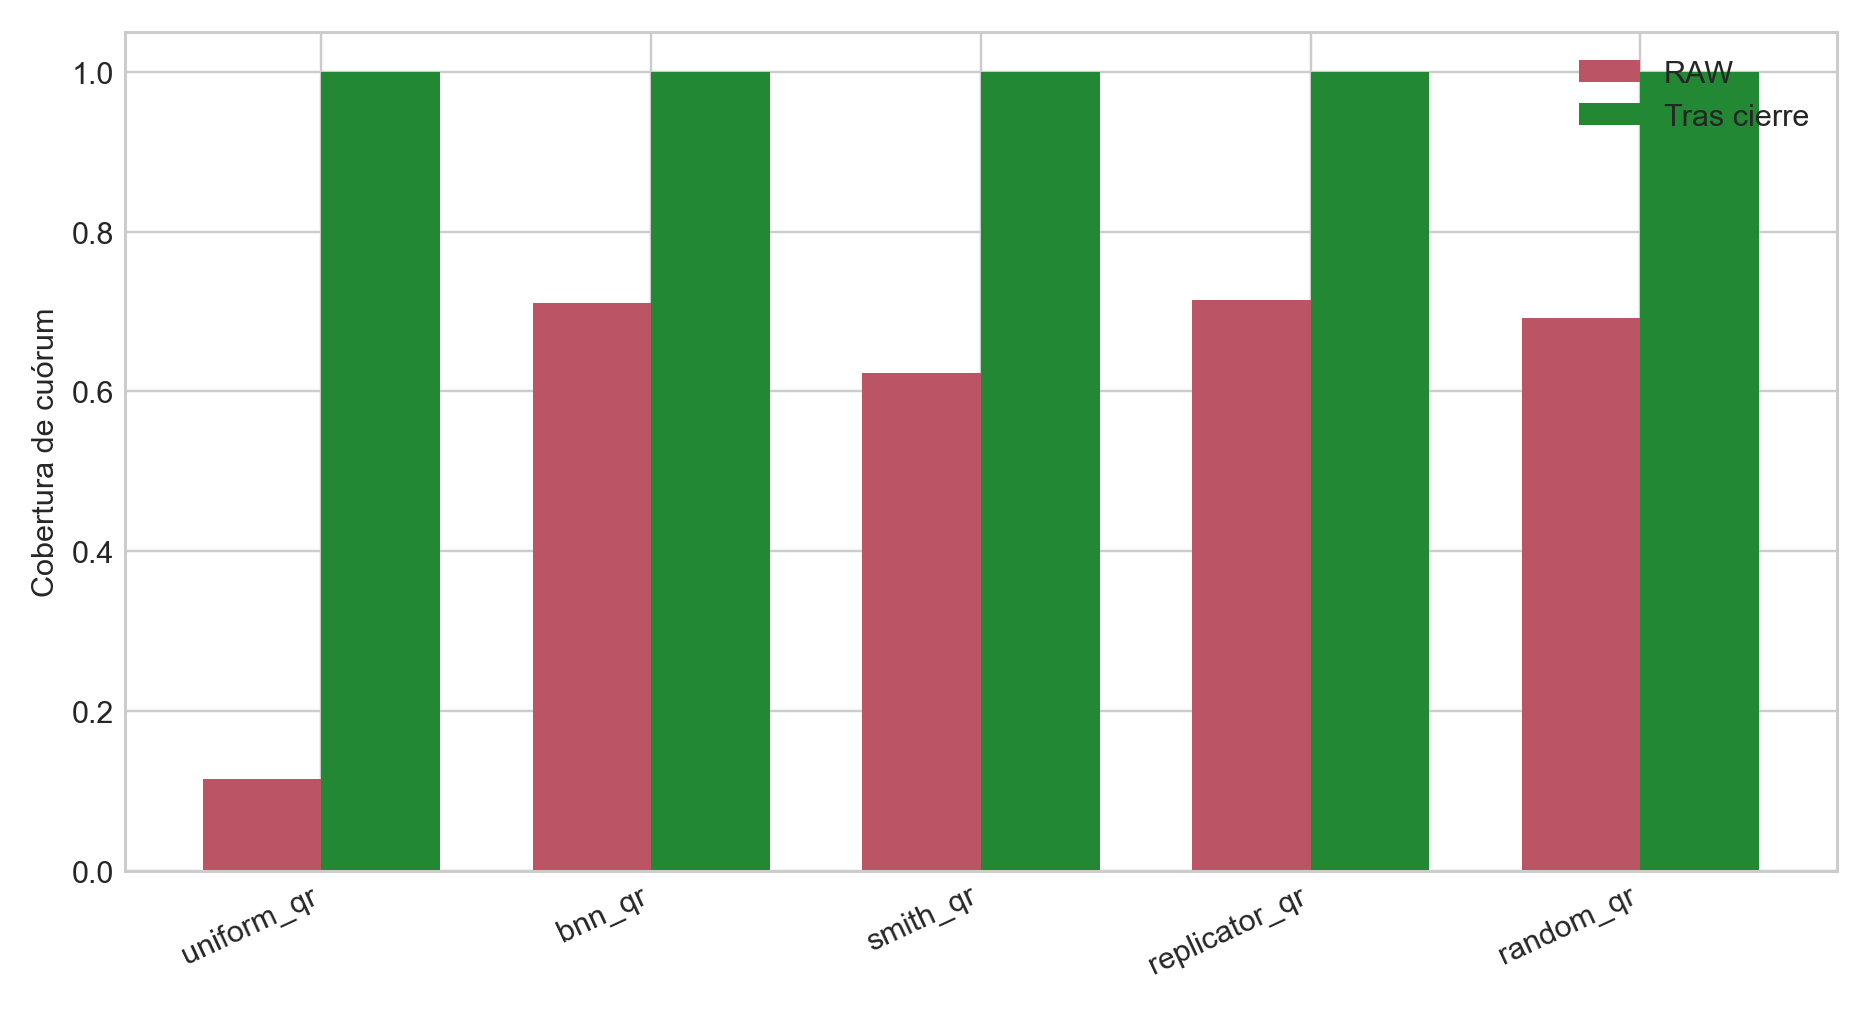
\includegraphics[width=\linewidth]{figures/fig-sp1-homogeneous-raw-closed.png}
\end{minipage}
\caption[Calidad y efecto del cierre en SP1]{Regret frente al óptimo y separación entre preferencia RAW y coalición CLOSED.}
\viuownsource
\label{fig:sp1-homogeneous-main}
\end{figure}

\subsubsection{Resultados}

La auditoría canónica terminó en PASS: error máximo del símplex
$6{,}66\times10^{-16}$, residuos finitos, mundos correctamente emparejados,
asignaciones RAW y CLOSED inmutables y separadas, y cero violaciones de potencial.
Todos los métodos alcanzaron validez final porque los que producían preferencias
fraccionarias compartieron el mismo cierre entero. Esa igualdad no debe leerse como
convergencia del juego: Smith fue válido antes del cierre solo en $1{,}67\%$ de los
mundos y cubrió en RAW una fracción media de $0{,}624$.

\begin{table}[H]
\centering
\scriptsize
\begin{tabularx}{\textwidth}{@{}p{0.22\textwidth}rrrrr@{}}
\toprule
Método & RAW válido & Cobertura RAW & Regret & Conv. & Mensajes \\
\midrule
Húngaro exacto & 1,000 & 1,000 & 0,0000 & 1,000 & 224 \\
Subasta proxy & 1,000 & 1,000 & 0,0298 & 1,000 & 224 \\
Uniforme+QR & 0,000 & 0,115 & 0,0444 & 1,000 & 16 \\
BNN+QR & 0,054 & 0,711 & 0,0514 & 0,503 & 715788 \\
Smith+QR & 0,017 & 0,624 & 0,0597 & 0,346 & 815898 \\
Greedy & 1,000 & 1,000 & 0,0808 & 1,000 & 16 \\
Replicador+QR & 0,011 & 0,715 & 0,0862 & 0,693 & 312795 \\
Aleatorio+QR & 0,003 & 0,692 & 0,4660 & 1,000 & 16 \\
\bottomrule
\end{tabularx}
\caption{Resultados agregados de 900 mundos por método. ``Conv.'' es el criterio numérico al horizonte, no una prueba asintótica.}
\label{tab:sp1-homogeneous-summary}
\end{table}

Smith+QR redujo el regret frente a greedy en $0{,}0212$ (IC95\% pareado
$[-0{,}0284,-0{,}0141]$, $p_{\rm Holm}<0{,}001$) y frente al control aleatorio
en $0{,}4064$. Sin embargo, la subasta proxy fue mejor por $0{,}0299$
(IC95\% $[0{,}0236,0{,}0358]$), y uniforme+QR fue mejor por $0{,}0153$
(IC95\% $[0{,}0092,0{,}0214]$, $p_{\rm Holm}=0{,}0029$). La brecha de Smith
respecto al óptimo fue $0{,}0597$. Todos los contrastes sobrevivieron Holm.

\begin{figure}[H]
\centering
\begin{minipage}[t]{0.49\textwidth}
\centering
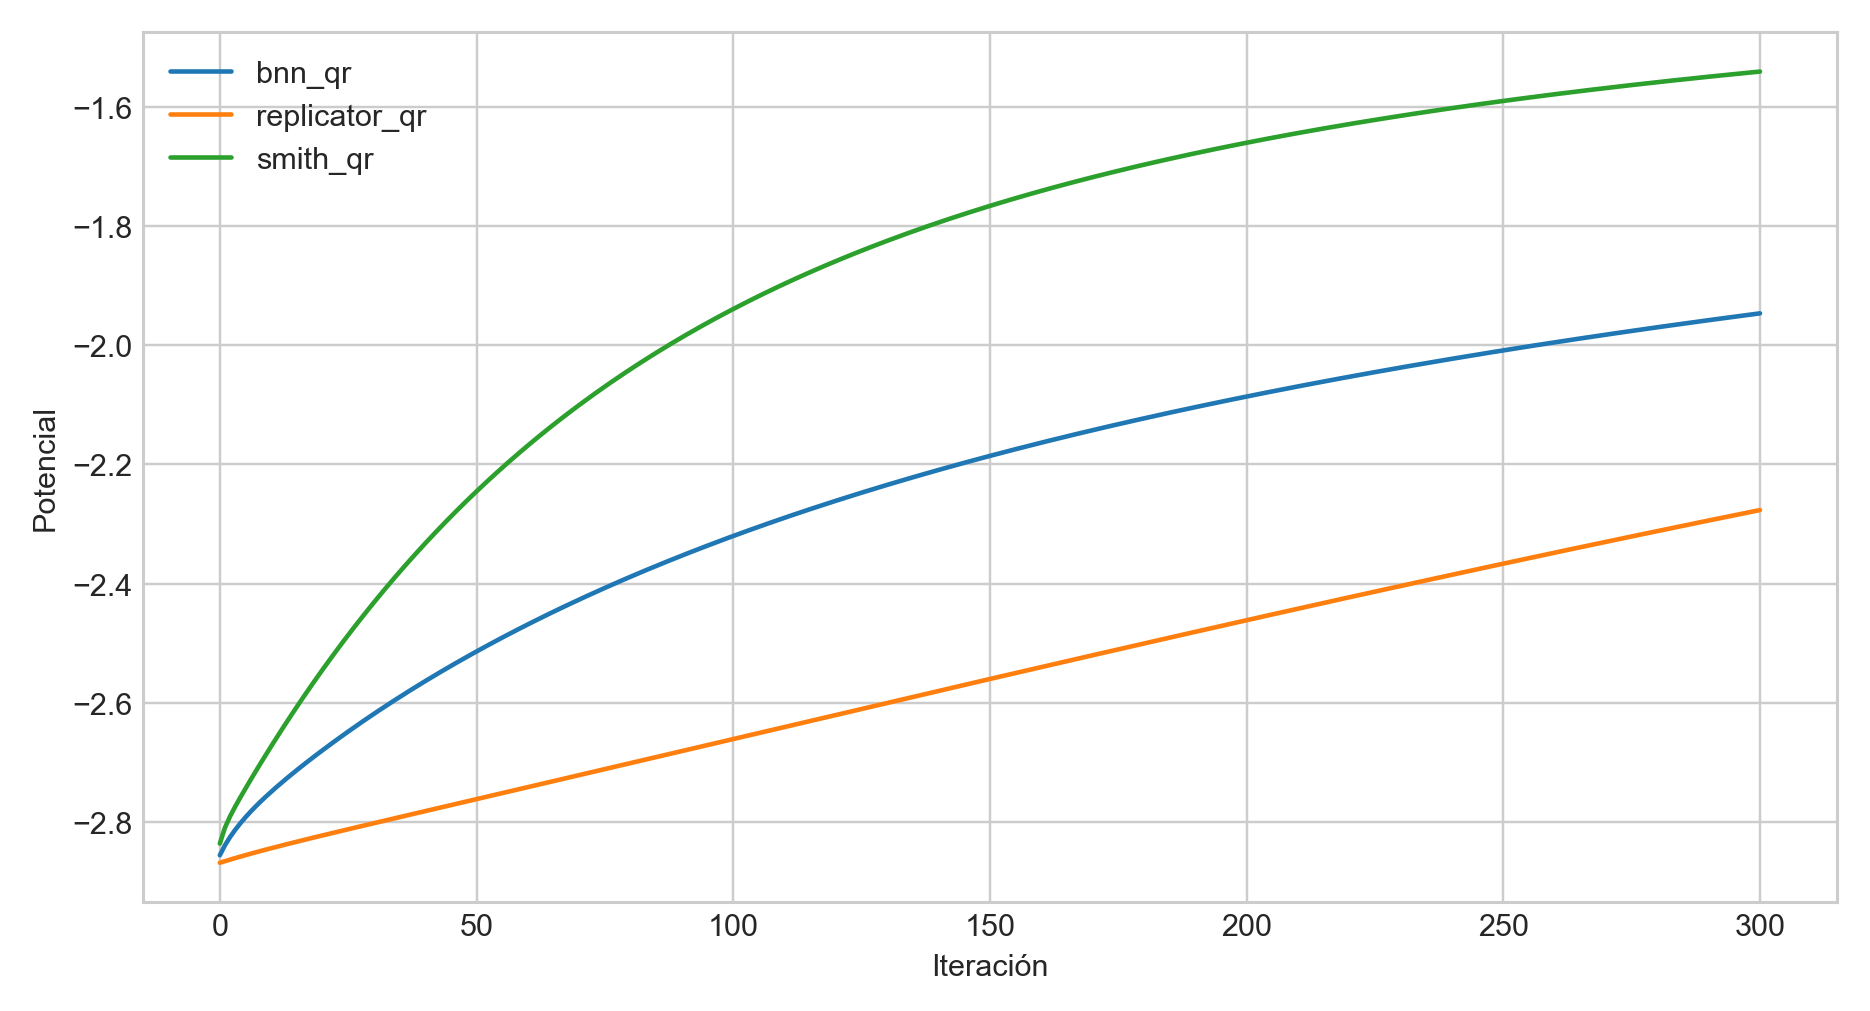
\includegraphics[width=\linewidth]{figures/fig-sp1-homogeneous-potential.png}
\end{minipage}\hfill
\begin{minipage}[t]{0.49\textwidth}
\centering
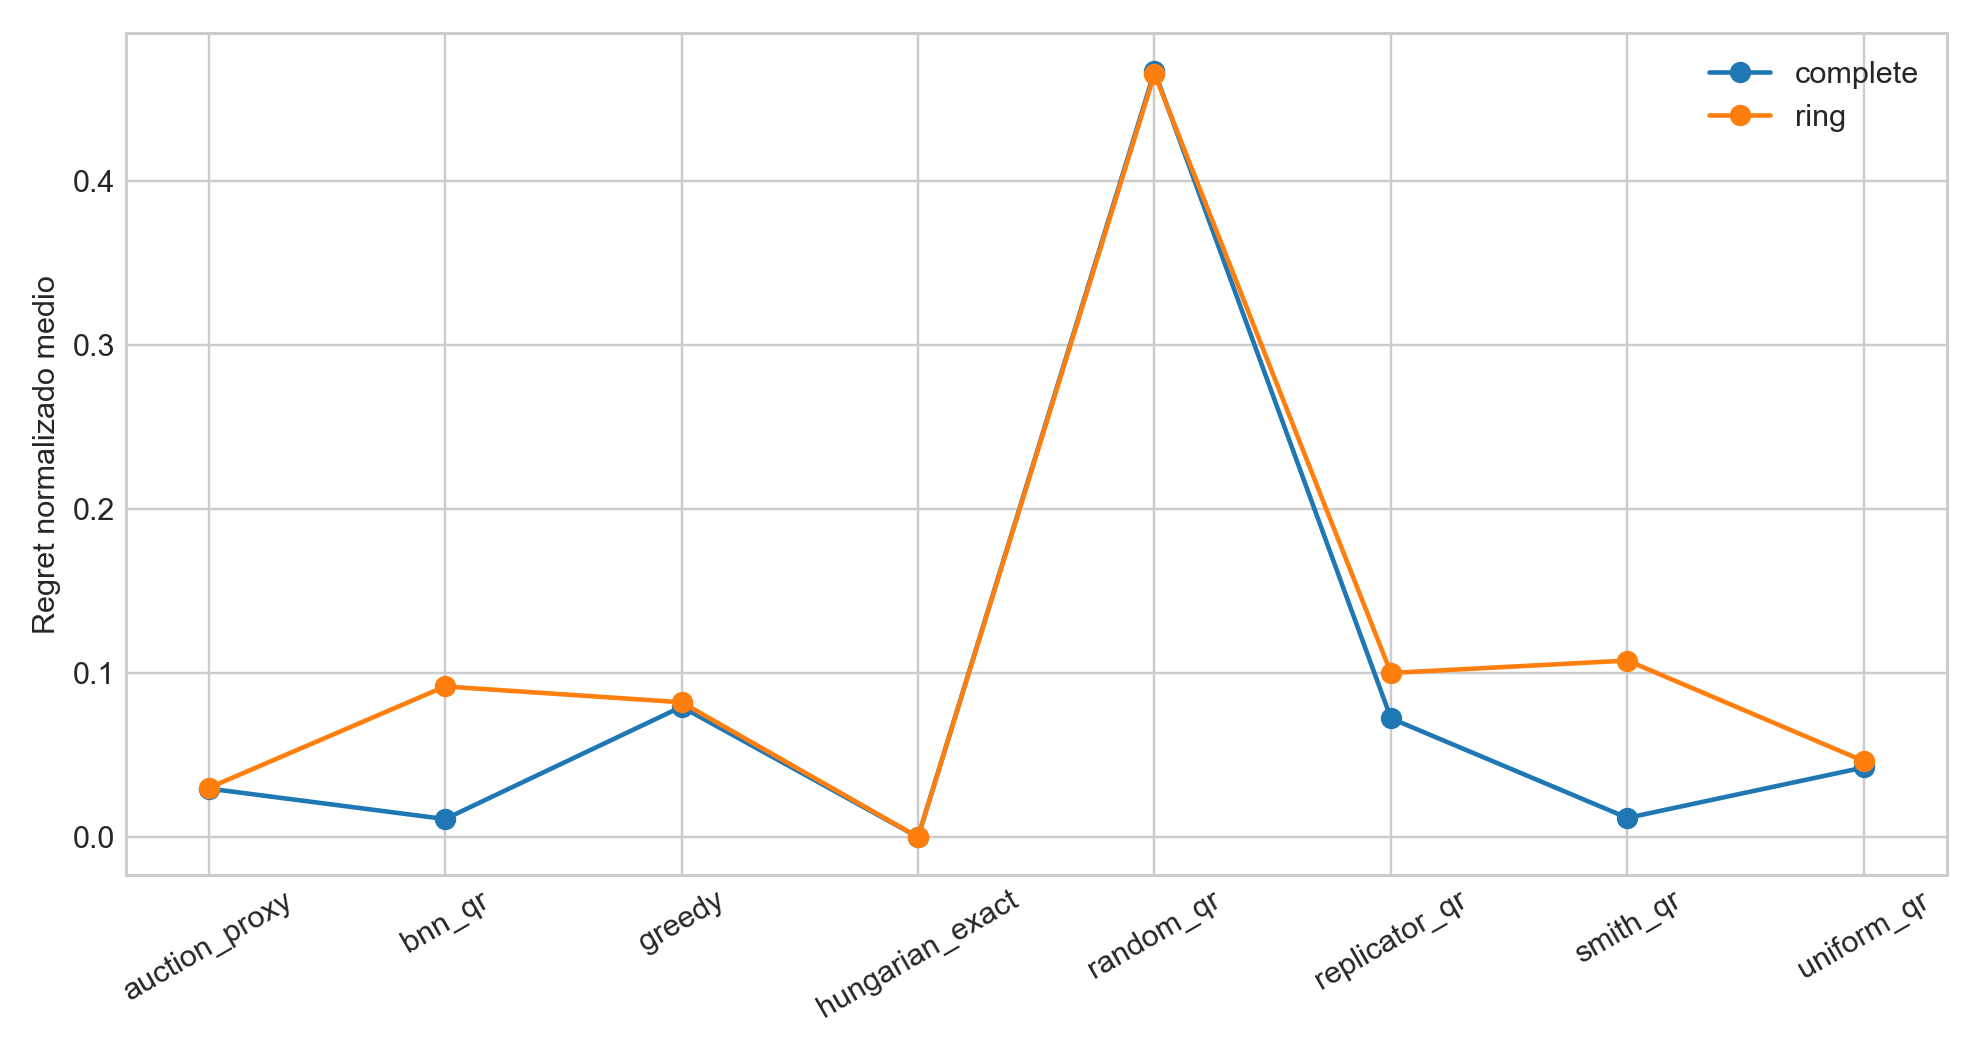
\includegraphics[width=\linewidth]{figures/fig-sp1-homogeneous-graph.png}
\end{minipage}
\caption[Potencial y sensibilidad al grafo en SP1]{Ascenso del potencial y degradación bajo estimación finita en anillo.}
\viuownsource
\label{fig:sp1-homogeneous-theory}
\end{figure}

El grafo explica una limitación central. Con información completa, el regret de
Smith fue $0{,}0117$; en anillo subió a $0{,}1076$. BNN pasó de $0{,}0110$ a
$0{,}0918$ y el replicador de $0{,}0724$ a $0{,}1000$. Estos datos no prueban
robustez a grafos variables: muestran que cuatro rondas de consenso en un grafo
fijo disperso no bastan para reproducir el juego de información exacta.

\paragraph{Conclusión exigente de SP1.}
El capítulo cierra cuatro resultados teóricos: invariancia del símplex, potencial
exacto, ascenso de Smith y terminación factible del cierre. También aporta un
protocolo reproducible que separa juego, decodificación y factibilidad. No demuestra
que Smith encuentre el óptimo entero ni que el sistema completo sea distribuido:
el cierre QR usado para validar cardinalidad dispone de preferencias globales. El
resultado uniforme+QR revela además que buena parte del rendimiento procede del
cierre. Por tanto, SP1 respalda la formulación mediante juegos poblacionales y su
trazabilidad, pero rechaza una narrativa de superioridad general frente a métodos
clásicos. La siguiente contribución debe distribuir el cierre o incorporar la
restricción entera en el propio juego antes de extender la afirmación a robótica
móvil ejecutable.
